\clearpage

\section{Simulation Analysis}
\label{sec:simulation}

\subsection{Operating Point Analysis - The Circuit for $t<0$}

Table~\ref{tab:sim1} shows the simulated operating point results for the circuit under analysis, for $t<0$.

 

\begin{table}[htb!]
  \centering
  \begin{tabular}{|l|r|}
    \hline    
    {\bf Name} & {\bf Value [A or V]} \\ \hline
    @gb[i] & -2.48284e-04\\ \hline
@r1[i] & 2.369027e-04\\ \hline
@r2[i] & -2.48284e-04\\ \hline
@r3[i] & -1.13810e-05\\ \hline
@r4[i] & 1.210640e-03\\ \hline
@r5[i] & -2.48284e-04\\ \hline
@r6[i] & 9.737374e-04\\ \hline
@r7[i] & 9.737374e-04\\ \hline
v(1) & 5.185042e+00\\ \hline
v(2) & 4.941554e+00\\ \hline
v(3) & 4.425830e+00\\ \hline
v(5) & 4.977013e+00\\ \hline
v(6) & 5.729012e+00\\ \hline
v(7) & -1.97652e+00\\ \hline
v(8) & -2.95469e+00\\ \hline
v(9) & 0.000000e+00\\ \hline

  \end{tabular}
  \caption{Operating point results. A variable preceded by @ is of type {\em current}
    and expressed in Ampere; other variables are of type {\it voltage} and expressed in
    Volt.}
  \label{tab:sim1}
\end{table}

These results and the ones that follow in this section were produced using the \textit{Ngspice software}.

For this range of time, the circuit is time static, which means that the Capacitor C behaves as an open circuit. This is shown in Figure \ref{fig:sim1}.
As well as that modification, we also had to add a new Independent Voltage Source with a voltage of 0V whose current would be $I_d$, in order for \textit{Ngspice} to recognise the Current-Controlled Voltage Source, defined in Figure \ref{fig:sim1} as $H_d$. Bearing this in mind the Voltage Source was added between node 0 and a new node 9, with node 9 being placed between the GROUND and the first terminal of $R_6$.

 

\begin{figure}[h] \centering
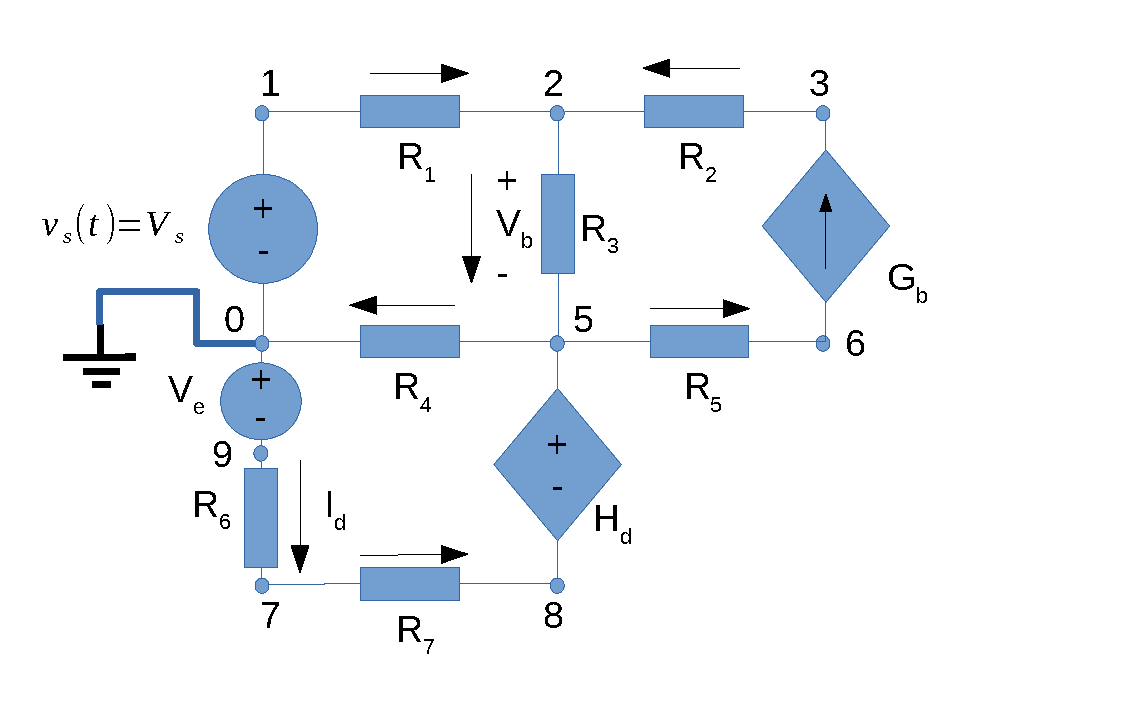
\includegraphics[width=0.6\linewidth]{t2-sim1.pdf}
\caption{The original circuit at $t < 0$ with an added voltage source of value 0V.}
\label{fig:sim1}
\end{figure}




\newpage

\subsection{Operating Point Analysis - Finding the Inital Conditions}

In this section, we analyse the following circuit:

 

\begin{figure}[h] \centering
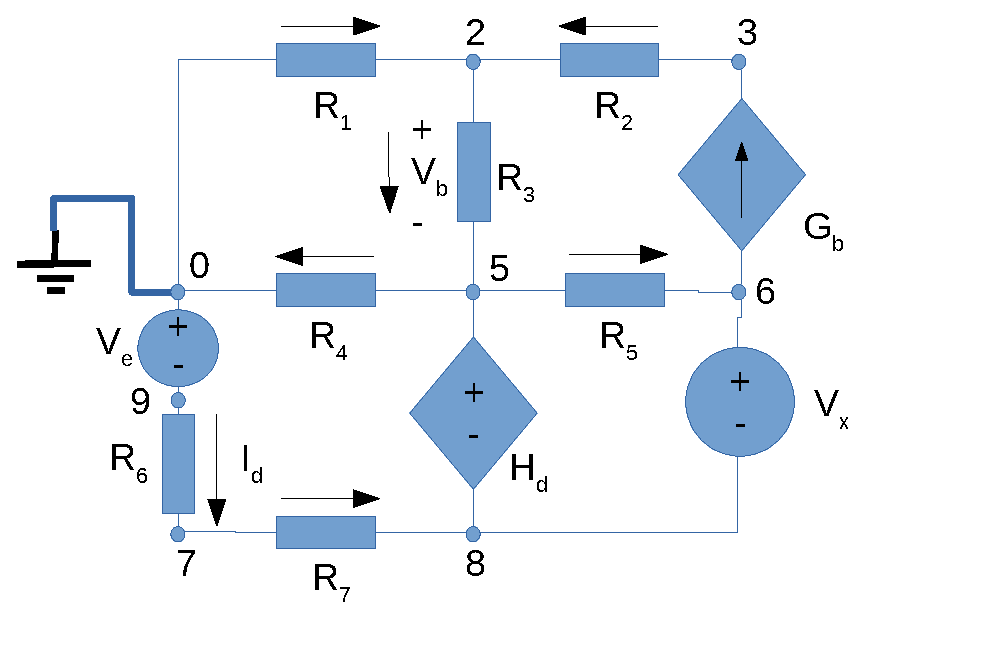
\includegraphics[width=0.5\linewidth]{t2-sim2.pdf}
\caption{The original circuit with an added voltage source of value 0V.}
\label{fig:sim2}
\end{figure}

Once again, the 0V Source is added for Ngspice to be able to recognise $H_d$.
Analysing this circuit is useful for us to be able to find the inital conditions of the original circuit at $V_6$ and $V_8$, the nodes that the Capacitor is connected to. We need this information because, from now on, the analysis of the circuit will be time-dependent and we need to know the inital conditions for the circuit.

The results for the Operating Point Analysis are represented in Table \ref{tab:sim2}.

 

\begin{table}[htb!]
  \centering
  \begin{tabular}{|l|r|}
    \hline    
    {\bf Name} & {\bf Value [A or V]} \\ \hline
    @gb[i] & 3.571179e-18\\ \hline
@r1[i] & -3.40748e-18\\ \hline
@r2[i] & 3.571179e-18\\ \hline
@r3[i] & 1.636985e-19\\ \hline
@r4[i] & 7.278356e-19\\ \hline
@r5[i] & -2.86705e-03\\ \hline
@r6[i] & 5.854099e-19\\ \hline
@r7[i] & 5.854099e-19\\ \hline
v(2) & 3.502198e-15\\ \hline
v(3) & 1.092010e-14\\ \hline
v(5) & 2.992175e-15\\ \hline
v(6) & 8.683696e+00\\ \hline
v(7) & -1.18828e-15\\ \hline
v(8) & -1.77636e-15\\ \hline
v(9) & 0.000000e+00\\ \hline

  \end{tabular}
  \caption{Operating point results. A variable preceded by @ is of type {\em current}
    and expressed in Ampere; other variables are of type {\it voltage} and expressed in
    Volt.}
  \label{tab:sim2}
\end{table}

As expected, these results give us the values we were looking for: $V_6 = 8.683696V$ (which equals $V_6(t < 0) - V_8(t < 0)$), and $V_8 \approx 0$ (which, compared to the size of $V_6$, we can assume is actually 0).



\clearpage

\subsection{Transient Analysis - No Forced Frequency}

For our first time-dependent analysis, we analyse the original circuit in the interval $t \in [0, 20]ms$, with no forced frequency, adding onto it, once again, the 0V Source:

 

\begin{figure}[h] \centering
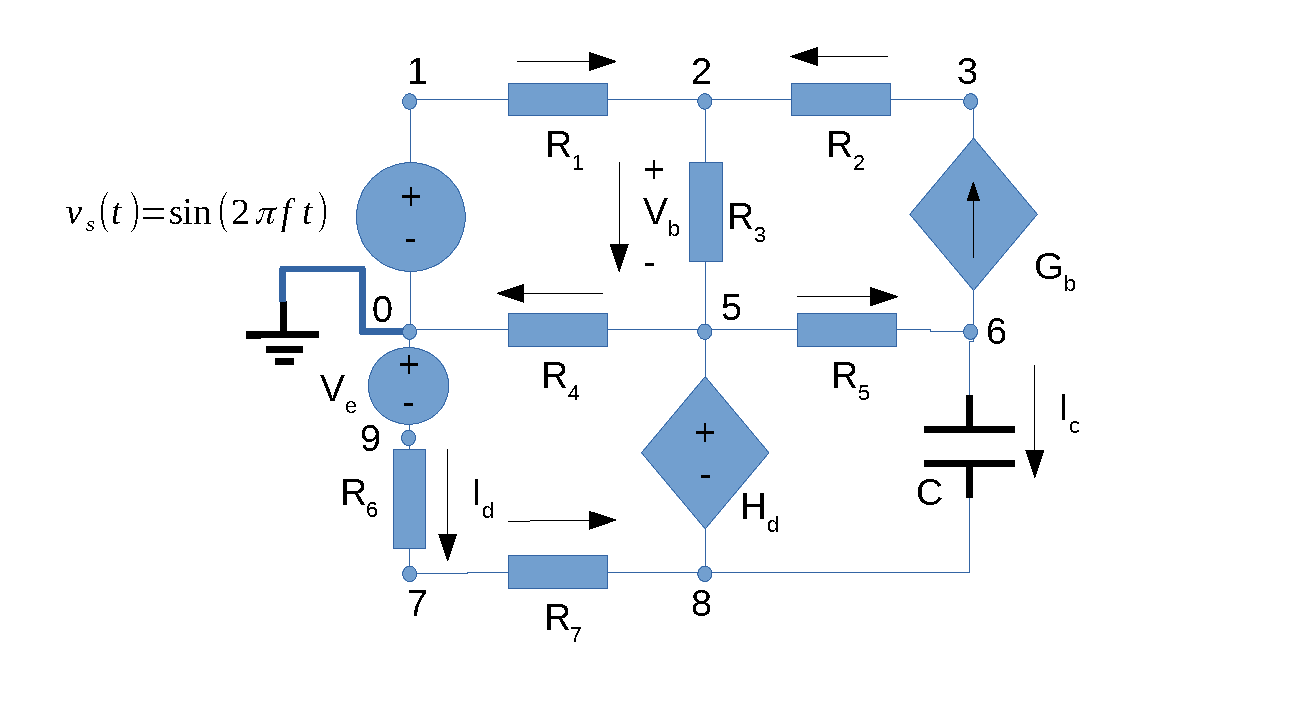
\includegraphics[width=0.7\linewidth]{t2-sim345.pdf}
\caption{The original circuit with an added voltage source of value 0V.}
\label{fig:sim345}
\end{figure}

This schematic of the circuit is the one that will also be followed in the next two sections.

For this analysis, we used the boundary conditions for $V_6$ and $V_8$ obtained in the previous section, with the AC Independent Voltage Source $V_s$ following a sinusoidal signal, displayed in Figure \ref{fig:sim345}. Considering the values obtained by \textit{Octave} and \textit{Ngspice} are the exact same until the 5th decimal number for both $V_6$ and $V_8$, we used the values obtained by \textit{Octave}, as that was an easier way to automate the production of this report. The same was done in the following sections as well. The result of the Transient Analysis made by \textit{Ngspice} is shown in Figure \ref{fig:sim-graph3}.

 

\begin{figure}[h] \centering
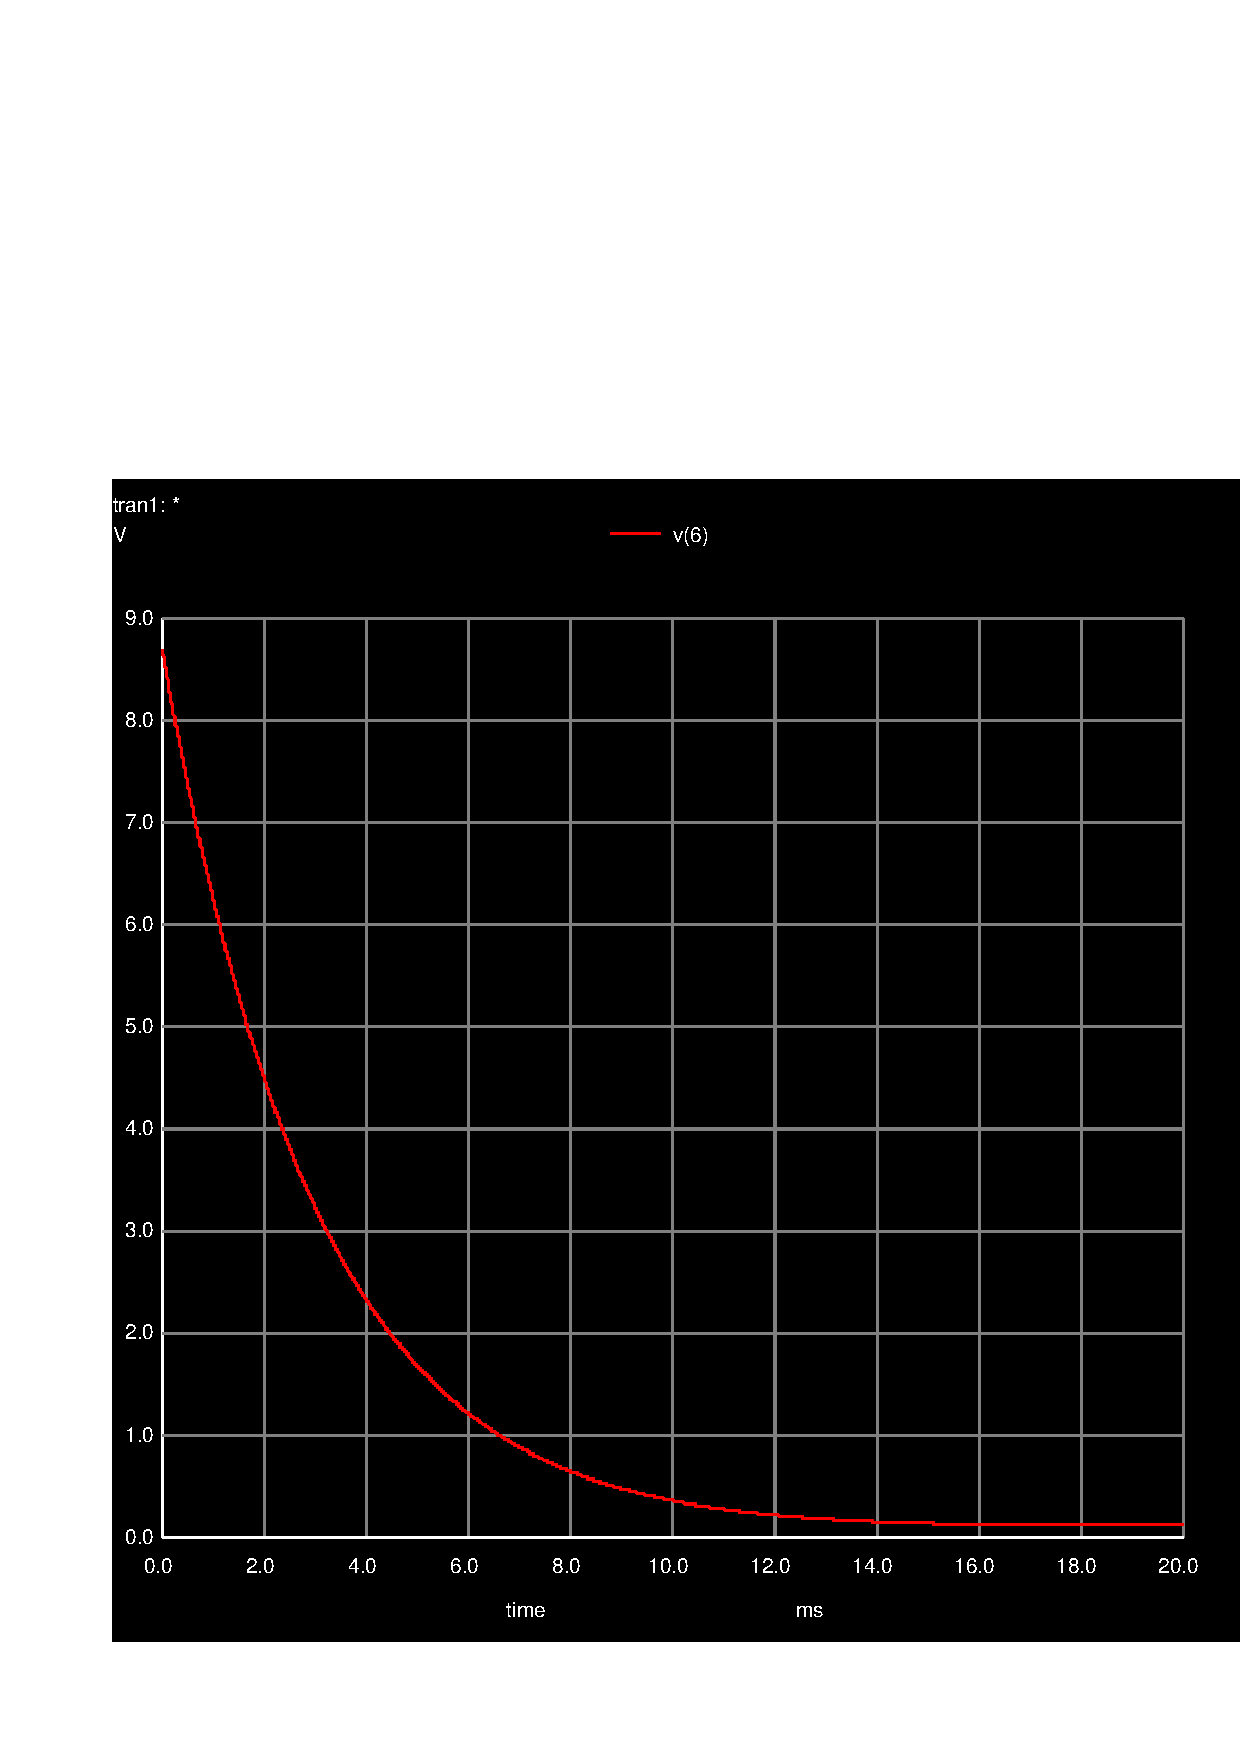
\includegraphics[width=0.4\linewidth]{../sim/trans3.pdf}
\caption{Voltage of $V_6$ (V) vs. Time ($\in [0, 20]ms$) - Transient Analysis of the Original Circuit with No Forced Frequency}
\label{fig:sim-graph3}
\end{figure}

As expected, the voltage of $V_6$ decays exponentially, as the Capacitor stores more and more energy as time goes by.


\newpage

\subsection{Transient Analysis - Forced Frequency of 1kHz}

In this section, we repeat the exact same steps taken in the previous one, except we introduce a forced frequency signal of 1kHz on $V_s$. In Figure \ref{fig:sim-graph4}, we can observe the stimulus and the response in node 6.


\begin{figure}[h] \centering
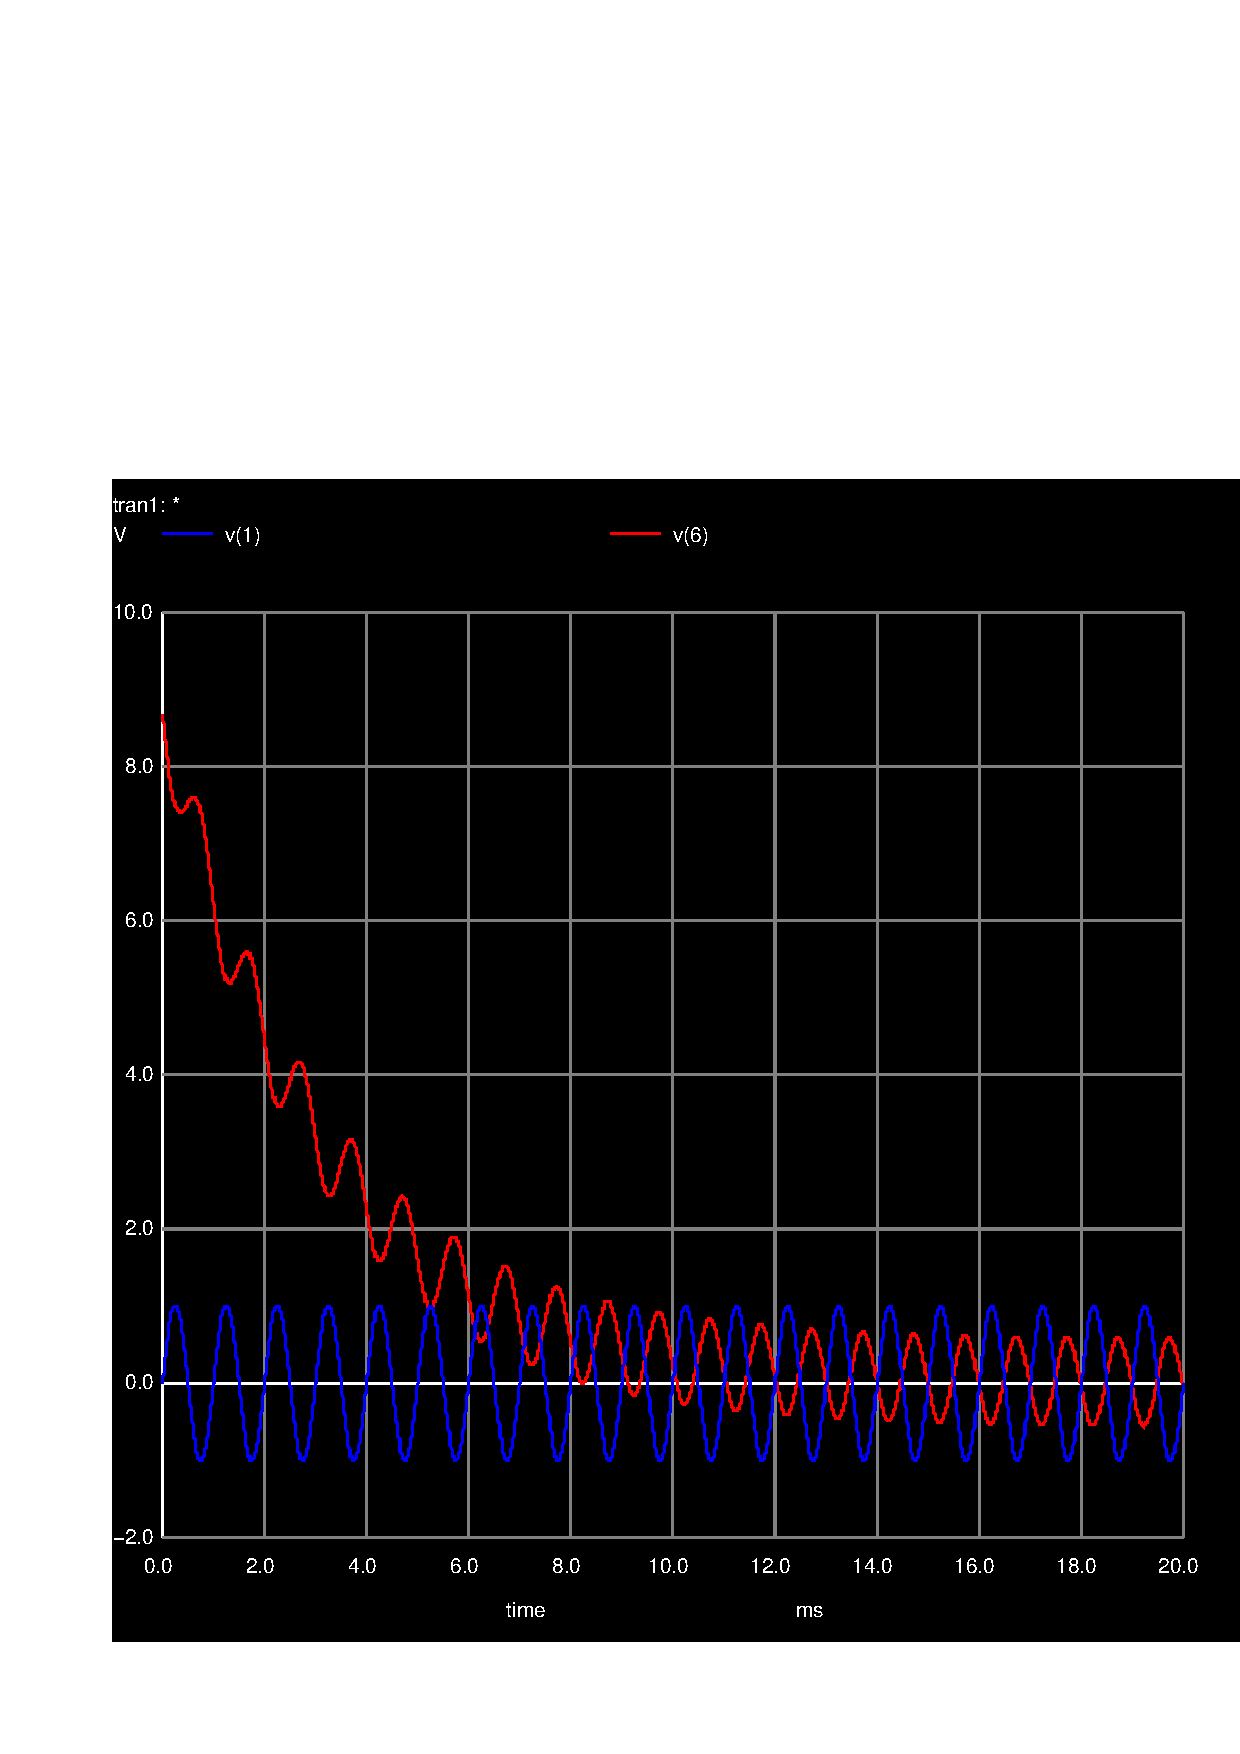
\includegraphics[width=0.4\linewidth]{../sim/trans4.pdf}
\caption{Voltage of $V_6$ and of the stimulus (V) vs. Time ($\in [0, 20]ms$) - Transient Analysis of the Original Circuit with a Forced Frequency of 1kHz}
\label{fig:sim-graph4}
\end{figure}

It is clear that the shape of $V_6(t)$ is the same as before, only now modulated by the stimulus, represented in Figure \ref{fig:sim-graph4} in blue, with the label v(1), because the voltage in node 1 is made up of a difference in potencial in the GROUND (whose volatge is 0) and by the voltage created by $V_s$.



\subsection{Frequency Analysis}

We now look at the original circuit in a range of forced frequencies of 0.1Hz to 1MHz. In Figure {fig:sim-graph5db}, we can observe the Amplitudes of $V_6$, $V_s$ and $V_c$ in dB, respectively represented by db(v(6)), db(v(1)) and db(v(6) - v(8)), as a function of the logarithm of the ranges of frequencies previously mentioned.


\begin{figure}[h] \centering
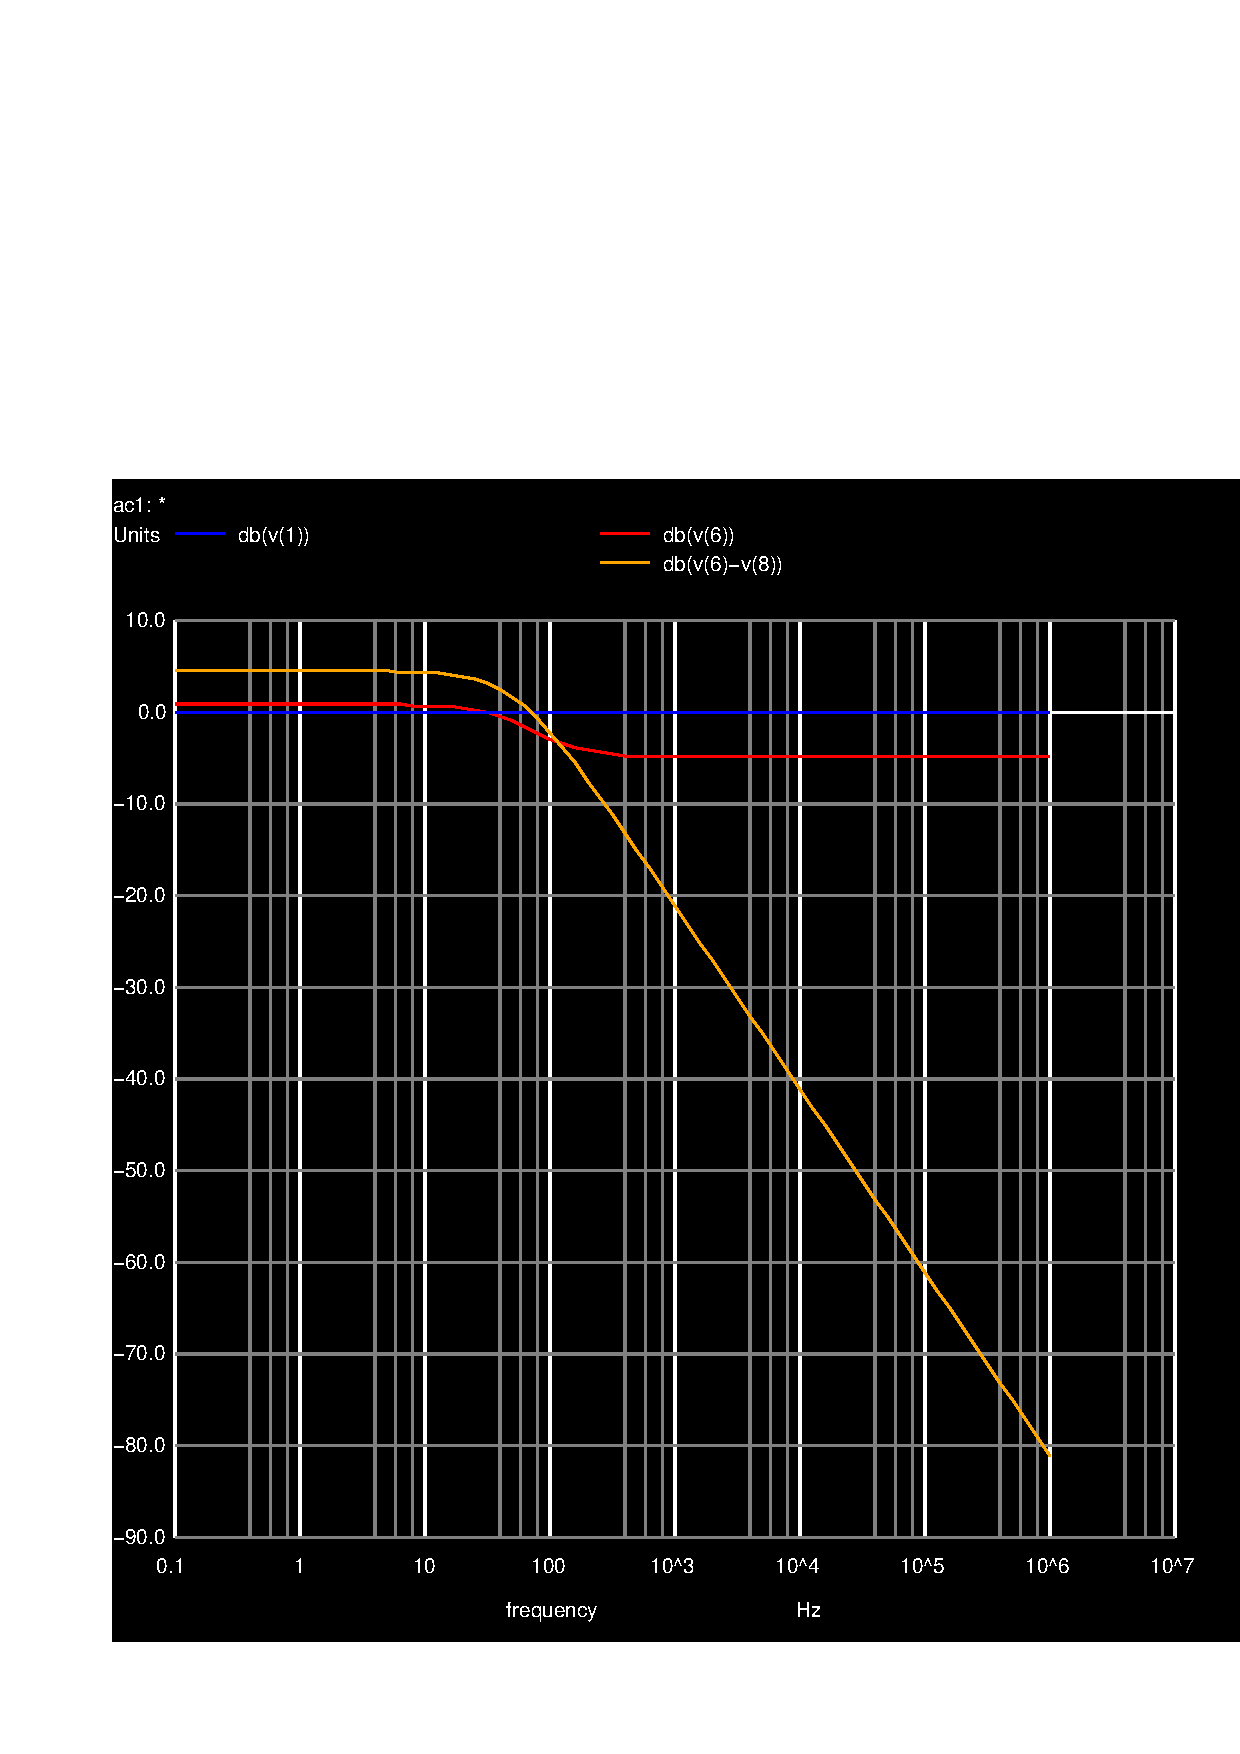
\includegraphics[width=0.4\linewidth]{../sim/db.pdf}
\caption{Amplitude of $V_6$, $V_s$ and $V_c$ (dB) vs. Frequency (Hz) - Frequency Analysis of the Original Circuit}
\label{fig:sim-graph5db}
\end{figure}

The first thing that the reader might notice is that the amplitude of $V_s$ is always zero. This happens because $V_s$ is the voltage source, so it mantains its amplitude constant throughout frequency changes, unlike $V_6$. It is zero because the amplitude would be 1 in Volts, but, transforming the units into dB, we have to do the base 10 logarithm of the amplitude in Volts, which results in an amplitude in dB of zero.

Lastly, we take a look at the phase of $V_6$, $V_s$ and $V_c$, respectively ph(v(6)), ph(v(1)) and ph(v(6) - v(8)), as a function of the same range of frequencies in Figure \ref{fig:sim-graph5ph}.

\begin{figure}[h] \centering
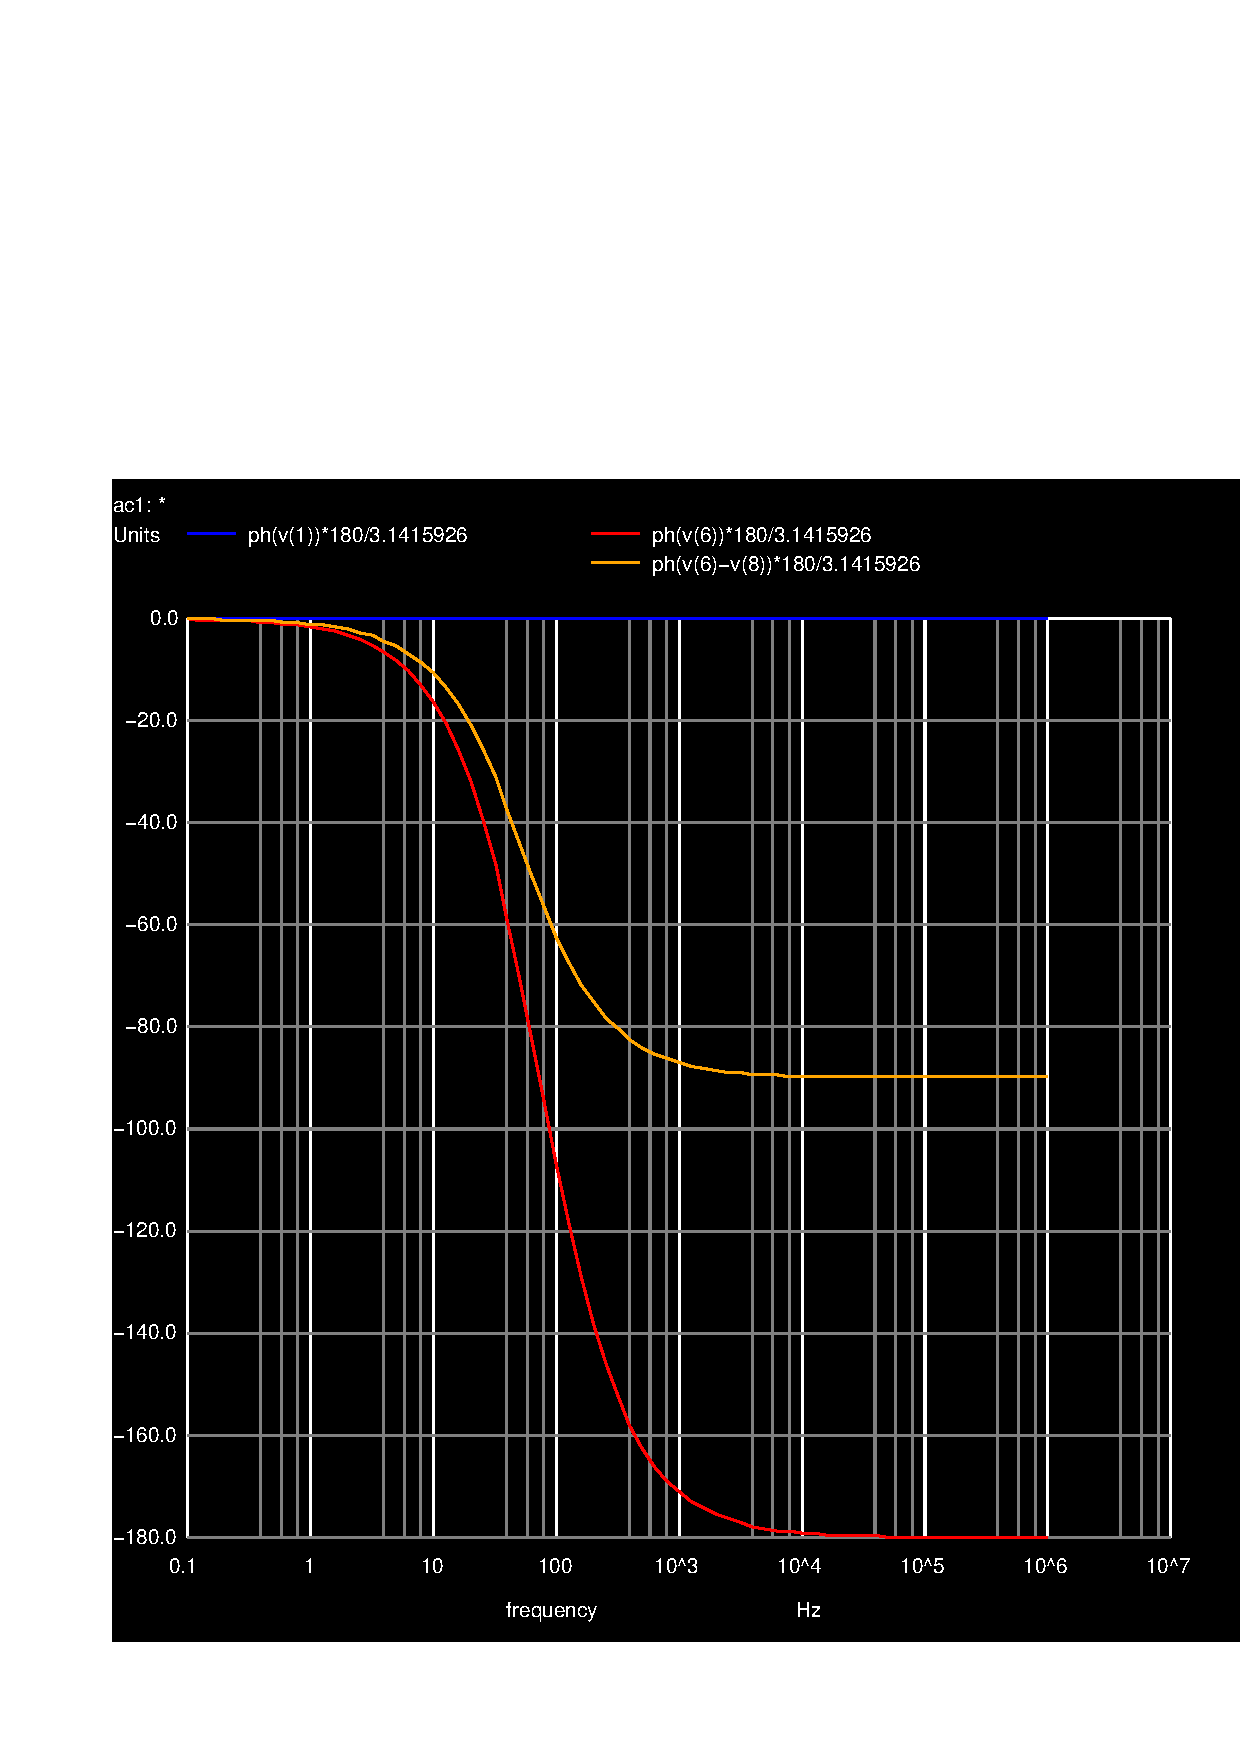
\includegraphics[width=0.4\linewidth]{../sim/ph.pdf}
\caption{Phase of $V_6$, $V_s$ and $V_c$ (degrees) vs. Frequency (Hz) - Frequency Analysis of the Original Circuit}
\label{fig:sim-graph5ph}
\end{figure}


As we can observe, all of the phases are 0 at $f=0.1Hz$ and then vary according to the frequency. Looking at the whole plot, particularly at the graph of the phase of $V_s$, we can assume that \textit{Ngspice} calculates the phase as (value for the fase at a certain node - value for the phase of the Voltage Source).